\section{Using GNS3. Practical Case Study}
\label{sec:gns3practicalcasestudy}

Here, we describe the process and results of the experiments carried out to assess aspects of the feasibility, and convenience, of using GNS3 in a computer networks course comprising the use of network gear on (emulated) network configurations.

Hopefully, some of the gained insights can be extrapolated for other similar teaching facilities of slightly different characteristics.

To provide a real and well-defined set of examples to put in practice, the selected exercises and lab descriptions were taken out of the lab classes handouts for the 2018-2019 edition of ``Architecture and Protocols of Computer Networks,'' known by its Portuguese acronym APRC, an elective, graduate course offered at the Masters in Informatics at the FCT/NOVA.

\subsection{Overview of the Considered Labs and Exercises}
\label{subsec:gns3consideredlabs}

Out of the 5 lab assignments, some of which span across more than one class, planned for a semester, only the first ones, which resort to the lab equipment to put in practice the subjects related to layer-2 and 3 switching, and ``legacy'' routing, as opposed to \gls{sdn}, were considered. % TODO "span across?". Usar esta nota para pôr, se tiver ficado esquecido, referência no trabalho futuro aos exercícios de SDN que podem tirar partido de GNS3 e afins. SDN tem tem de estar nos acrónimos e glossário
Those are the exercises that, in the present, are expected to be done in the lab room, with real interconnected Cisco devices, issuing commands to the IOS command-line interface from the students' laptops.

The so-called ``lab-assignment1'' has a part to introduce the Cisco IOS and some basic commands for it.
Those are the ones to enter and escape the privileged mode, list the device's interfaces, and some other queries.
It also informs of how to load the running configuration of the device into the non-volatile memory, so that it persists after a shutdown, and how to do the opposite to discard unsaved running configurations and load the ones from the nonvolatile memory.

The second handout, ``lab-assignment2,'' is all about switching and layer-2 functionality.
It proposes a topology, expected to map the real interconnecting and physical disposition of devices in the room, of the nine switches, labels them with ``areas'' corresponding to cardinal points.
Students are then guided to answer questions about the expected behavior, e.g. in terms of reachability between hosts, according to parameters, which they should also issue in a coordinated fashion, for STP, VLANs, and trunks.

For the third lab assignment, divided into two parts, students are requested to connect their laptops to a topology similar to the one in the switching labs, but setting up the network interfaces on the nine multi-layer devices that interconnect them as layer-3 routing nodes.
As written in the handout, the idea is that the routers interconnect the backbone of the offices of a nation-wide corporation.
Therefore, the computers in each bench (office), have its interface in different IP prefixes, corresponding to separate LANs. % TODO add gls reference

First, to set up set routing, students are requested to design an addressing plan, setting up prefixes and hosts on the routing interfaces connected each router to another, and then setup manually, using IOS's interface, static routes that allow to connect each office's LAN to another.
After this, students can configure the router/switch virtual interface (which is also configured to be on its respective LAN) as the default gateway and \texttt{ping} each other's computer.

The second goal is to, instead of doing the routing statically, configure the routers to use OSPF, and perform a set of analysis and variations on the exercise, such as changing the bandwidth of some links, turning other links off and foreseeing the behavior according to the specification of the protocol.

Students are also requested to use Wireshark to capture the data OSPF exchanges across the network.

\subsection{Testing Environment}
\label{subsec:environment}

Testing with GNS3 was done running the GNS3 server in virtual machines on DI's servers, except for some experiments with Dynamips carried out on an Apple laptop. % TODO acronyms?
The virtual machines are machines with two Intel Xeon E5-2650~v4~@~2.20~GHz (a total of 24 cores) and 64~GiB of RAM.
The two virtual machines used to test the lab handouts' topologies are running on the VMware ESXi bare metal hypervisor, with nested virtualization enabled (needed so appliances, which are themselves VMs, can be emulated), had 4 CPU cores, and 2 and 8 GB of RAM allocated, respectively.
The laptop is a MacBook Pro with a 6-core Intel Core~i7~@~2.20~GHz and 16~GiB of RAM.
Exercises with IOSv were first tried out in the aforementioned laptop, but it was impossible to even start the nodes and have them functional.

For the switching labs, all the nodes of the topology were set to run on the same machine.
Conversely, for the sake of testing that functionality, the routing (static and OSPF) labs were tested with the nodes distributed across two computes (both on the infrastructure previously described).

% Figure fig:gns3-aprc-lab2-handout-topology
\begin{figure}
  \centering
  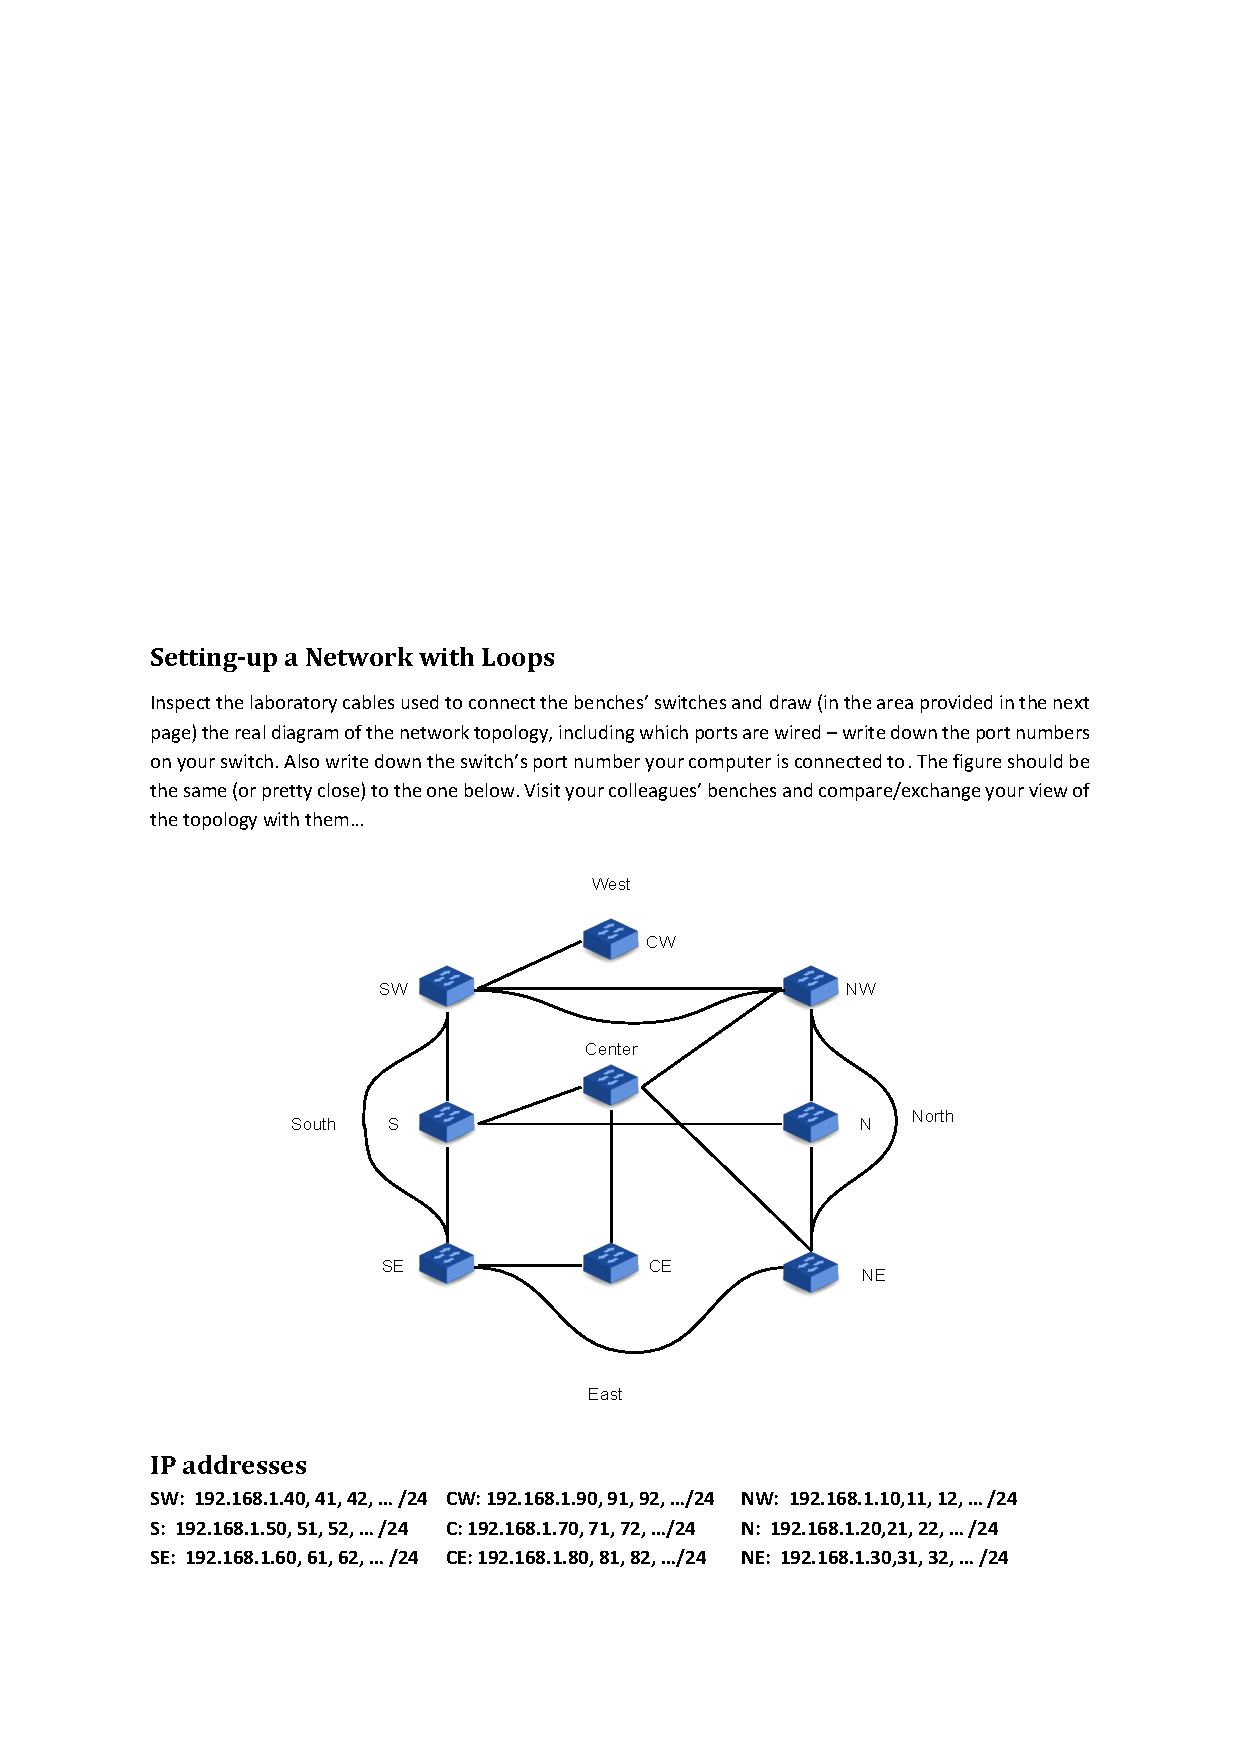
\includegraphics[width=0.8\textwidth, frame]{gns3-aprc-lab2-handout-topology}
  \caption{Section of ``lab-assignment2'' showing the topology}
  \label{fig:gns3-aprc-lab2-handout-topology}
\end{figure}


\subsection{Introduction to Cisco IOS and Switching Labs}
\label{subsec:gns3introswitching}

As stated earlier, the first lab assignment introduces host-side commands (mostly Linux) and TCP/IP practical concepts such as IP address and \acrshort{mtu}, and its definition for the host's \acrfullpl{nic}.
The part of this lab handout that is to be performed on Cisco is perfectly doable on a GNS3 session with both (lighter) Dynamips EtherSwitch-enabled legacy routers or the more modern Cisco IOSvL2-3.
Double clicking on a node corresponding to one of these switches/routers, the GNS3 GUI will launch a terminal window on the user's desktop automatically executing the command necessary to create a \texttt{telnet} session to the node.

To perform the second lab, the topology described in figure~\ref{fig:gns3-aprc-lab2-handout-topology} (a section of the handout document) is physically implemented in the lab room with Cisco Catalyst switches interconnected accordingly with UTP-Ethernet cables supporting the data links.
The topology has loops which STP, running in the switches, is expected to eliminate by disabling certain link(s).
Part of the exercise is to foresee, according to the protocol's specification, which one(s) will be shutdown.

Execute this exercise in GNS3 already poses a bit of challenge, and introduces a dilemma.

IOSvL2, as mentioned earlier, runs on QEMU/KVM, which is only supported on GNU/Linux computes.
On a laptop setup with macOS or Windows the standard GNS3 installation recommends having VMware Fusion or Workstation, respectively, installed and downloading the so-called GNS3 VM, which nothing else than a VM image, optimized for VMware's desktop hypervisors, containing a pre-made installation of the GNS3 server on an Ubuntu Server LTS.
The GNS3 GUI for macOS and Windows then facilitates setting up the ``GNS3 VM'' to not need to setup a generic remote server to be used as compute, and is also able to open VMware Fusion or Workstation in the background and power on the GNS3 VM, as a means to offer a standardized compute node.
Needless to say, this does not come without its overhead, both in terms of performance and practicality.

On the other hand, using a Dynamips EtherSwitch, that can be run directly on a macOS or Windows installation, and is much, much lighter, is not recommended anymore, since it requires legacy Cisco images, may not provide all the functionality, is reported to have bugs, etc.

In practice, though, if students have access to the IOS images compatible with the school's labs switches, all the exercises were proven to be performable on a laptop using Dynamips nodes.
VLANs are supported by these images, as well as STP, and standard routing protocols, such as OSPF (covered on a lab assignment too) are also run without problems on these equipments.

Summarizing, using Dynamips is no longer (officially) encouraged.
However, one assumes that the advice seen on the GNS3 forums, and on the videos and interviews with Jeremmy Grossmann already cited, for not using Dynamips is very much centered on advanced features and IOS interface compatibility.
However, in an undergraduate or graduate university level, where applying theoretical principles and seeing and doing in practice, in a controlled environment, not bound to any vendor tools, this advice may very well be irrelevant.

% Table tab:gns3-iperf
\begin{table}
  \centering
  \small
  \begin{tabulary}{0.9\textwidth}{ll}
    \toprule
      \textbf{Network appliance}     & \textbf{Throughput between two nodes}\\
    \midrule
      Cisco c3745 (Dynamips process) & $\approx 191~\mbox{Mbit/s}$\\
      Cisco IOSvL2 (KVM via QEMU)    & $\approx 66~\mbox{Mbit/s}$\\
    \bottomrule
  \end{tabulary}
  \caption{%
    Approximate average throughput between two Docker Ubuntu Guest appliances connected to two different network node implementations, measured with \texttt{iperf3} and a total 1024~MiB of transfered data.
  }
  \label{tab:gns3-iperf}
\end{table}


That said, Dynamips ensures actually better throughput on its EtherSwitch modules between two hosts connected to the same device than an analogous scenario with IOSvL2 switches.
It also is dramatically lighter on resource consumption, and users can emulate such nodes on their macOS or Windows---and obviously on GNU/Linux, which supports GNS3's emulation alternatives fully, too---without having any need for a distributed or load balanced architecture.

Table~\ref{tab:gns3-iperf} compares the results of measuring the throughput of two Docker Ubuntu Guest appliances connected to the same switch.
The emulated nodes were all in the same compute node, so no traffic between separate hosts was necessary.
That data, for IOSv was obtained in the campus infrastructure environment, described above, while, for a Dynamips EtherSwitch, the test was performed in both the infrastructure and the laptop, yielding virtually the same results.
Another observed value was the memory used by each Dynamips process while running the \texttt{iperf3} command, which was very close for all cases---Docker guests, Cisco c3745 with EtherSwitch module, and IOSvL2---all between 99~MiB and 112~MiB.

\subsection{Routing and OSPF on Cisco Routers}
\label{subsec:gns3ospfrouting}

Although the considerations related to using Dynamips versus using IOSv are also applicable here, the complexity of this exercise will be used to demonstrate two facets of GNS3's functionality and setup-wise flexibility, namely:
\begin{itemize}
  \item Distributing the load between many servers (computes)---useful to scale, and particularly necessary when emulating heavier nodes such as IOSv instances.
  \item Topology snapshots
\end{itemize}

For a large topology, since GNS3's emulation is quite heavy (more details on that later), distributing the load may be necessary to make an emulation feasible.
GNS3's topologies are JSON files describing which devices exist on it, their names, meta-information to be used in the moment where each emulator is executed, and which links connect which virtual interfaces~\cite{thebookofgns3}.
Therefore, there is not a practical limitation for the central points, the controller and the GUI, in the size which a topology can have.
It is possible, and examples across the web are given, of enormous topologies.

The real burden is on the computes, which symbolize each host where virtual routers and guests run.
To \textbf{distribute the load}, one uses separate hosts to run an instance of the GNS3-server, in the role of a compute, receiving instructions from the controller (in turn controlled by the user using, for instance, the GNS3 GUI) to interact with the running emulators.
As long as the total amount of emulators and ubridge processes attached to those processes running on each of those hosts doesn't use too many resources of each compute-host, there isn't exactly any bottleneck (obviously, apart from the \emph{real} networking connectivity between the compute hosts of nodes in the topology), since the emulated nodes execute independently of GNS3's ``brains''.

Unless the user is editing the topology, creating or deleting nodes and links, starting and stopping machines, or other orchestration-specific tasks, the interaction with the running nodes is done thought direct \texttt{telnet} connections to the emulator processes from terminal windows accessible to the user, outside of GNS3.
To make that easier, if using the GNS3 GUI, a user can double click on e.g. a ``powered-on'' switched or Ubuntu Docker Guest, and a helper is transparently executed which will open a terminal window on that (graphical) host, automatically running a command like \texttt{telnet 10.170.138.106 5001}---where \texttt{10.170.138.106} is the IP address of the compute host where a certain node is running and \texttt{5001} is the concrete TCP port where the emulator process is listening to accept connections to the console.

In the case of the lab assignment 3 (layer-3 routing and OSPF), the (virtual) servers were set up in the way illustrated by figure~\ref{fig:gns3-ospf-lb}.
One was running the GNS3 server as the controller (and also as compute for some nodes), and the other only as a ``secondary'' compute node.
Note that there is no reason to assume that the ``primary'' (generally, the controller) is the host with the most resources.
In fact, this wasn't the case in the architecture set up for this experiment.

The \textbf{topology snapshots} functionality of GNS3 can be extremely useful for incremental laboratory handouts, where certain ``checkpoints'' must be achieve.
Instructors may setup certain parameters in advance and record snapshots.
Snapshots contain any kind of current state not only of the topology/project configuration at GNS3's level itself (in the role of the orchestrator, link simulation parameters like package loss rate, etc.) but also the persisted state of emulated devices, like Dynamips or IOSv routers, which allows playing with the IOS settings much more easily, including with the \texttt{copy ...}-family commands.

% Figure fig:gns3-ospf-lb
\begin{figure}
  \centering
  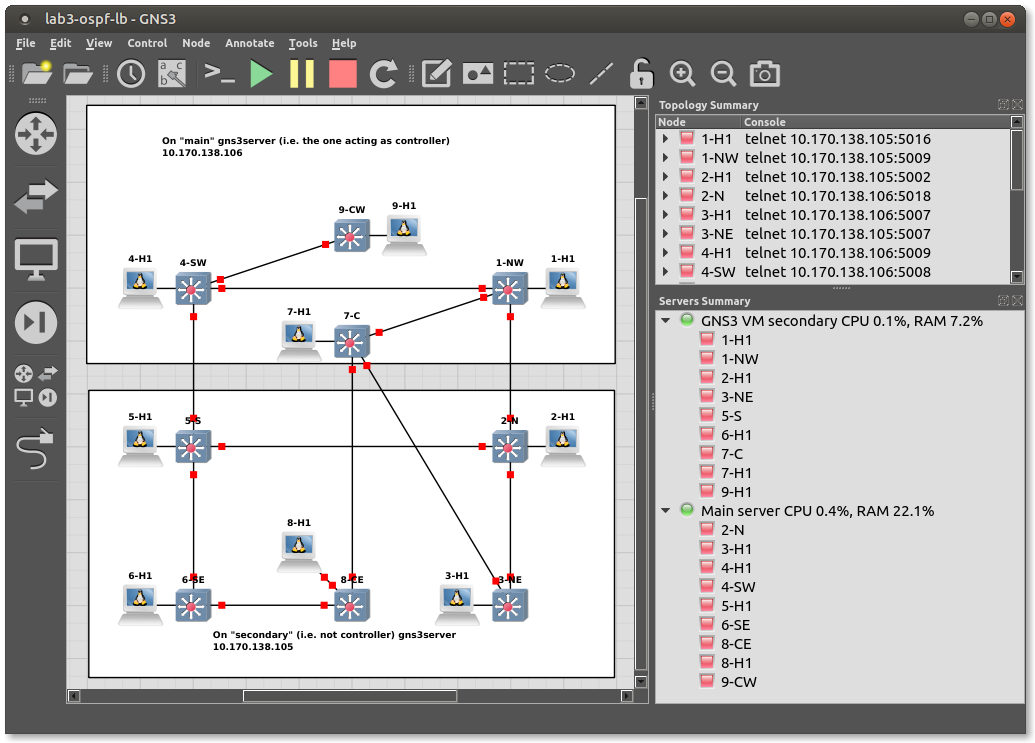
\includegraphics[width=0.9\textwidth]{gns3-ospf-lb}
  \caption{View of load-balanced lab~3's topology in GNS3 GUI}
  \label{fig:gns3-ospf-lb}
\end{figure}


% end of section gns3practicalcasestudy
